% Article for documents at The Hague University
% of Applied Sciences, Dept. of Electrical Engineering.
%
% (c)2021, J. op den Brouw <J.E.J.opdenBrouw@hhs.nl>
%
% Added 22-01-2014: failure feature 4 and 5 if analysis fails.
% Added 05-03-2014: changed tmf file name.
% Added 08-03-2014: minor spelling corrections.
% Added 09-03-2014: new screenshot BDF Conversion
% Added 18-09-2018: update script + VBS script to install the flow
% Added 27-08-2021: update script
%

%% 12pt charachters, A4 paper size, one side printing, equation left aligned
%% equation indent at 0 em
\documentclass[11pt,a4paper,final,oneside,titlepage,fleqn]{article}

%% Set input encoding to UTF-8
\usepackage[utf8]{inputenc}
%% Use T1 output font encoding
\usepackage[T1]{fontenc}

%% PDF Version and compression...
%\pdfminorversion=5
%\pdfobjcompresslevel=2

%% Paragraph
\usepackage{parskip}

%% English spelling of chapter, section, etc.
\usepackage[english]{babel}

%% Set page layout
\usepackage[a4paper,bindingoffset=0.2in,left=1in,right=1in,top=1in,bottom=1.4in,footskip=0.4in]{geometry}
\addtolength{\skip\footins}{10pt}
\setlength{\headheight}{13.6pt}

%% Allows increasing the font size of specific fonts beyond LaTeX default specifications
%\usepackage{anyfontsize}

%% Use appendix
%%\usepackage{appendix}

%% Use of dashed lines in tables
%\usepackage{arydshln}

%% Create text-wrapped figures and tables
%\usepackage{wrapfig}

%% Include graphics files
\usepackage{graphicx}

%% Enumerate items
\usepackage{enumitem}

%% Use the AMS Mathematical characters
%\usepackage{amsmath}
%\usepackage{amsfonts}
%\usepackage{amssymb}
%\setlength{\mathindent}{1em}

%% Use computer code listings
\usepackage{listings}

%% Use Biber as BibLatex backend
\usepackage[
    backend=biber,
    backref=true,
    backrefstyle=none,
    sortcites=true,
    sorting=none,
    doi=false, % doi informatie wordt niet weergegeven
    %uniquename=true,
    %uniquelist=true,
    maxcitenames=1,
    %issn=false, werkt niet
]{biblatex}
\addbibresource{convertBDFtoVHDL.bib}

%% Do not show ISSN numbers
\AtEveryBibitem{\clearfield{issn}}
\AtEveryCitekey{\clearfield{issn}}

% Use Charter for Roman and Nimbus Mono for TT
\usepackage{charter}
\usepackage{nimbusmono}

%% Fancy headers and footers...
\usepackage{fancyhdr}
\pagestyle{fancy}
\lhead{}
\chead{}
\rhead{CONCEPT}
\lfoot{Using ModelSim with Quartus II Block Design Files}
\cfoot{}
\rfoot{\thepage}
\renewcommand{\headrulewidth}{0pt}
\renewcommand{\footrulewidth}{0.4pt}

%\renewcommand{\footnoterule}{%
%  \kern -3pt
%  \hrule width \textwidth height 1pt
%  \kern 2pt
%}

%% Indexing words...
%\usepackage{makeidx}
%\makeindex

%% Making captions nicer...
\usepackage[font=footnotesize,format=plain,labelfont=bf,textfont=it]{caption}

%% For using footnotes in section headers...
\usepackage[stable]{footmisc}

%% Define and use colors
\usepackage{xcolor}
\definecolor{dkgreen}{rgb}{0,0.6,0}
\definecolor{gray}{rgb}{0.5,0.5,0.5}
\definecolor{mauve}{rgb}{0.58,0,0.82}
\definecolor{lightgray}{rgb}{0.95,0.95,0.95}

%% Using hyperrefs...
\usepackage{hyperref}
\hypersetup{
	colorlinks=true,
	linkcolor=blue,
	citecolor=dkgreen,
    pdftitle={Using ModelSim with Quartus II Block Design Files},
    pdfauthor={J.E.J op den Brouw},
    pdfsubject={A Block Design File to VHDL File converter and Modelsim Starter},
    pdfkeywords={Block Design File} {BDF} {Quartus} {ModelSim} {Tcl}
}
%\renewcommand\UrlFont{\fontfamily{phv}\selectfont\footnotesize}
%\renewcommand\UrlFont{\fontfamily{pcr}\selectfont}
\urlstyle{sf}

%%% No package loading from here


%% Def by Jean-Côme Charpentier
\lstdefinelanguage{tclfix}% from tcl definition
{alsoletter={.:,*=&-},%
morekeywords={after,append,array,names,exists,anymore,donesearch,%
get,nextelement,set,size,startsearch,auto_mkindex,binary,break,%
case,catch,cd,clock,close,concat,console,continue,default,else,%
elseif,eof,error,eval,exec,-keepnewline,exit,expr,fblocked,%
fconfigure,fcopy,file,atime,dirname,executable,exists,extension,%
isdirectory,isfile,join,lstat,mtime,owned,readable,readlink,%
rootname,size,stat,tail,type,writable,-permissions,-group,-owner,%
-archive,-hidden,-readonly,-system,-creator,-type,-force,%
fileevent,flush,for,foreach,format,gets,glob,global,history,if,%
incr,info,argsbody,cmdcount,commands,complete,default,exists,%
globals,level,library,locals,patchlevel,procs,script,tclversion,%
vars,interp,join,lappend,lindex,linsert,list,llength,lrange,%
lreplace,lsearch,-exact,-regexp,-glob,lsort,-ascii,-integer,%
-real,-dictionary,-increasing,-decreasing,-index,-command,load,%
namespace,open,package,forget,ifneeded,provide,require,unknown,%
vcompare,versions,vsatisfies,pid,proc,puts,-nonewline,pwd,read,%
regexp,-indices,regsub,-all,-nocaserename,return,scan,seek,set,%
socket,source,split,string,compare,first,index,last,length,match,%
range,tolower,toupper,trim,trimleft,trimright,subst,switch,tell,%
time,trace,variable,vdelete,vinfo,unknown,unset,uplevel,upvar,%
vwait,while,acos,asin,atan,atan2,ceil,cos,cosh,exp,floor,fmod,%
hypot,log,log10,pow,sin,sinh,sqrt,tan,tanh,abs,double,int,round,
foreach_in_collection,post_message,-submsgs%
},%
morestring=[d]",%
% MoreSelectCharTable=% <= the strange definition
% \lst@CArgX\#\relax\lst@DefDelimB{}{}%
% {\ifx\lst@lastother\lstum@backslash
% \expandafter\@gobblethree
% \fi}%
% \lst@BeginComment\lst@commentmode
% {{\lst@commentstyle}\lst@Lmodetrue}%
morecomment=[l]\# % <= this one ! Much simpler
}[keywords,comments,strings]%

\lstset{ %
  language=tclfix,                  % the language of the code
  basicstyle=\footnotesize\ttfamily,       % the size of the fonts that are used for the code
  commentstyle=\itshape,
  numbers=left,                   % where to put the line-numbers
  numberstyle=\tiny\color{gray},  % the style that is used for the line-numbers
  stepnumber=1,                   % the step between two line-numbers. If it's 1, each line will be numbered                           
  numbersep=5pt,                  % how far the line-numbers are from the code
  backgroundcolor=\color{lightgray},  % choose the background color. You must add \usepackage{color}
  showspaces=false,               % show spaces adding particular underscores
  showstringspaces=false,         % underline spaces within strings
  showtabs=false,                 % show tabs within strings adding particular underscores
  frame=lines,                   % adds a frame around the code
  rulecolor=\color{black},        % if not set, the frame-color may be changed on line-breaks within not-black text (e.g. comments (green here))
  tabsize=4,                      % sets default tabsize to 2 spaces
  captionpos=b,                   % sets the caption-position to bottom
  breaklines=true,                % sets automatic line breaking
  breakatwhitespace=false,        % sets if automatic breaks should only happen at whitespace
  title=\lstname,                   % show the filename of files included with \lstinputlisting;
  aboveskip=\bigskipamount,
}

%\lstset{ %
%  language=XML,                  % the language of the code
%  basicstyle=\footnotesize\ttfamily,       % the size of the fonts that are used for the code
%  commentstyle=\itshape,
%  numbers=left,                   % where to put the line-numbers
%  numberstyle=\tiny\color{gray},  % the style that is used for the line-numbers
%  stepnumber=1,                   % the step between two line-numbers. If it's 1, each line will be numbered                           
%  numbersep=5pt,                  % how far the line-numbers are from the code
%  backgroundcolor=\color{lightgray},  % choose the background color. You must add \usepackage{color}
%  showspaces=false,               % show spaces adding particular underscores
%  showstringspaces=false,         % underline spaces within strings
%  showtabs=false,                 % show tabs within strings adding particular underscores
%  frame=lines,                   % adds a frame around the code
%  rulecolor=\color{black},        % if not set, the frame-color may be changed on line-breaks within not-black text (e.g. comments (green here))
%  tabsize=4,                      % sets default tabsize to 2 spaces
%  captionpos=b,                   % sets the caption-position to bottom
%  breaklines=true,                % sets automatic line breaking
%  breakatwhitespace=false,        % sets if automatic breaks should only happen at whitespace
%  title=\lstname,                   % show the filename of files included with \lstinputlisting;
%  morekeywords={id,tasks,type},	%
%}

\title{Using ModelSim with Quartus II Block Design Files \\ \medskip\large A Block Design File to VHDL File Converter and ModelSim Starter}

\author{Jesse op den Brouw \\
	The Hague University Of Applied Sciences \\
    Department of Electrical Engeneering \\
	\medskip  \\
	\href{mailto:J.E.J.opdenBrouw@hhs.nl}{J.E.J.opdenBrouw@hhs.nl} \\
%	\bigskip \\
%	CONCEPT \\
	\bigskip
	}

\date{\today} 

%% Remove indention througout the document
%%\setlength\parindent{2em}

\begin{document}
\maketitle

\begin{abstract}
Students at The Hague University Of Applied Sciences get their first glimpse
at Digital Design education using only schematic entry using the Quartus II
software environment. Schematic entry is done using a full screen WYSIWYG
editor and generates Block Design Files (BDF files). This is a proprietary
file type and is not supported outside the Quartus II environment.

Simulation is at this stage unknown to them. We try to hide as much as
possible as not to distract their attention from the design process.

ModelSim is a full fledged VHDL and Verilog simulator and widely spread
amongst digital system designers, but is unable to compile and simulate
Quartus' BDF files.

Quartus provides an option to convert BDF files to VHDL files. Converting BDF
files to VHDL files is a tedious and error prone operation and has to be done
every time the design is updated.

This document describes a set of files as part of a \textit{design flow} that
deals with all of the problems mentioned above. The scripts run both on
Windows and Linux operating systems. Both the Subscription Edition and the Web
Edition are supported.
\end{abstract}

% create a table of contens 
\tableofcontents
\newpage
\lstlistoflistings
\listoffigures
\newpage

%%%%%%%%%%%%%%%%%%%%%%
\section{Introduction}
%%%%%%%%%%%%%%%%%%%%%%
\label{sec:introduction}
%%In Quartus, BDF files are a proprierity file type used
Students of the faculty of Electrical Engineering at the The Hague University
of Applied Sciences\footnote{In Dutch: De Haagse Hogeschool}~\cite{web/hhs} get
acquainted with digital design in the first year of their study. The learning
line consists of three courses.

In the first course they learn the basics of digital design like number systems,
boolean algebra, logic gates, K-maps and some elementary knowledge of latches
and flip-flops. At this stage, they do not use VHDL or any other HDL, and they
do not know anything about simulation.

For practical work, the students use the Quartus II design software from Altera.
As hardware platform, they use the DE0 Digital Systems Board supplied
by Terasic~\cite{web/terasic_de0}. It consists of a Cyclone III FPGA with about
15,000 cells, LEDs, switches, push buttons and seven segment displays. 

All the practical work in the first course is done using schematic entry and
using logic gates to complete the assignments. They do use hierarchies.
The students use simulation
but only to verify if their solution is correct; all the simulation scripts
and testbenches have been prepared by faculty staff.

Schematic designs are saved in so-called Block Design Files. Block Design Files
are proprietary files to Quartus. These files, recognizable by the extension
\texttt{.bdf}, can be synthesized using the Quartus software.

Simulation is done with Modelsim. ModelSim is a well known and widespread VHDL
and Verilog simulator, but is unable to compile and simulate BDF files.

Fortunately, Quartus has an option to convert BDF files to VHDL or Verilog files.
This can be done by opening the appropriate BDF file and using the Create HDL File
option. You can see a screenshot in Figure~\ref{010convertbdftohdl}.

\begin{figure}[!ht]
  \centering
  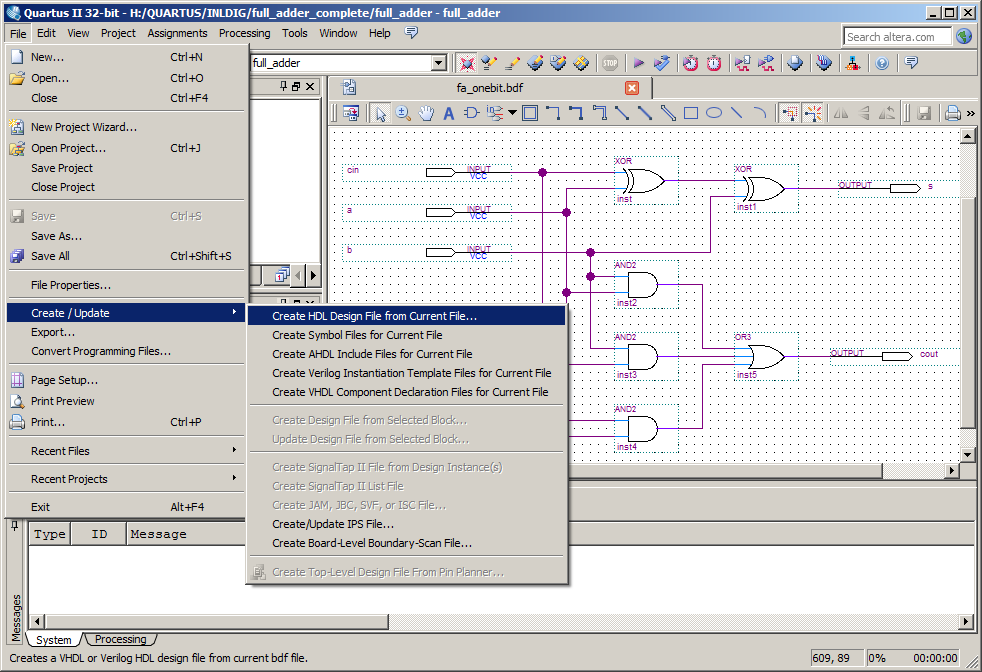
\includegraphics[scale=0.44]{010convertbdftohdl.png}
  \caption{Converting a Block Design File to an HDL File.}
  \label{010convertbdftohdl}
\end{figure}

Of course, this has to be done for every file in the project and every time
the files have changed. This is not only dull, but also error prone. You can
easily forget to convert a changed file, render the design useless.

This document describes a set of files that deals with all of the problems
mentioned above. There are two files: a script that handles the conversion of
Block Design Files to VHDL files and starts ModelSim automatically, and a file
that will set up the script as part of a so-called \textit{design flow}. The
files run both on Windows and Linux operating systems. Both the Subscription
Edition and the Web Edition are supported.

This document consists of eight sections. %%\regtotcounter{section}\total{section} sections.
Section~\ref{sec:projsetup} describes more about how a typical project is set
up.
Section~\ref{sec:environment} describes the environment the script runs in.
Section~\ref{sec:overview} contains a first description on what the scripts
actually does.
Section~\ref{sec:internal} gives an in-depth explanation of the script's
internal working.
Section~\ref{sec:modelsimcommandfile} gives some hints on how to set up a
generic ModelSim command file.
Section~\ref{sec:installation} describes the installation of the script and
the design flow file.
Section~\ref{sec:remember} gives some notes on things to avoid when
creating schematics.
At last, Section~\ref{sec:issues} deals about some known issues.

The intended audience are designers who make use of Block Design Files and
want to use ModelSim as their favorite simulator, and faculty staff who
want their students to use schematic entry of digital systems (and of course
use ModelSim for simulation).

Please note that the script hasn't been tested with Mega Functions or MaxII
functions, only with primitive functions such as AND, OR, and NOT.

There is a similar script for converting BDF files to Verilog files by Chris
Zeh. See~\cite{web/fixer}.


%%%%%%%%%%%%%%%%%%%%%%%%%%%%%%%%%%%%%%%%%
\section{A Typical Quartus Project Setup}
%%%%%%%%%%%%%%%%%%%%%%%%%%%%%%%%%%%%%%%%%
\label{sec:projsetup}
Before we tell more about the internals of the script it's best to give an
overview of a typical Quartus project suited for this setup.

For the script to work, there are two true obligations: the name of the
ModelSim command file must consist of the prefix \texttt{tb\_} followed by the
name of the top level design entity (which is not the design entity name of
the testbench) and the extension \texttt{.do}, and the name of the top level
design entity must be the same as the first part of the design filename.
There are really no other obligations (even the top level filename can
differ from the top level entity name, but it is included to force students
to use some sensible filenames).
Note that for BDF files, the name of the design entity is always the same as
first part of the filename. Also note that this is not always true for HDL
files. So if there's a top level design entity with the name
\texttt{full\_adder}, the corresponding filename must be
\texttt{full\_adder.bdf} (or \texttt{full\_adder.vhd} as an example).
It's good practice though to keep the filename of
the testbench as close as possible to the design entity filename, so the name
of the corresponding testbench filename should the same as the top level entity
name with the prefix \texttt{tb\_} and the extension \texttt{.vhd}. The typical
project has the following files:

\begin{itemize}[label=,itemsep=0pt]
\item \texttt{full\_adder.bdf} - the Block Design File with the top level design entity
\item \texttt{tb\_full\_adder.vhd} - the testbench file
\item \texttt{tb\_full\_adder.do} - the ModelSim command file
\end{itemize}

\noindent
It's possible to use hierarchies, consisting of multiple BDF files. The script
is able to process all BDF files in the current project. It's also possible
to incorporate more that one ModelSim command file to simulate multiple
(sub) designs. The only thing you have to do is to change the top level design
entity name in the Quartus environment (and run Analysis and Synthesis, see
Section~\ref{sec:issues}).

The project may contain other file types such as VHDL and Verilog files. The
script will not touch these files as long as they are not generated from BDF
files.

Only BDF files visible in the project environment (the files you see in the
Files tab of the Project Navigator in the Quartus IDE) are processed, all
other BDF files are not processed. 
Rationale for this is that you probably created the BDF file in the course of
the project and forgot to delete the file when is wasn't needed anymore.
Note however that all VHDL files associated with such BDF files are removed.
This way, ModelSim will not compile them when using the code in Listing~%
\ref{code:modcommand} in Section~\ref{sec:modelsimcommandfile} (and it
seems odd to have those VHDL files linger on).

It is possible to use a VHDL or Verilog file as the top level design entity.
When instantiating designs from BDF files, you can just use the design entity
names. Note that in the corresponding VHDL files, the architecture name is
always \texttt{bdf\_type}.

%%For the script to work, there must be a top level design entity that resides
%%in a file where the first part of the filename is the same a the name of the
%%top level entity. The extension should be \texttt{.bdf} for Block Design
%%Files. So if there's a top level entity with the name \texttt{full_adder},
%%the corresponding filename must be \texttt{full_adder.bdf}. The name of
%%the corresponding testbench filename should the same as the top level entity
%%name with the prefix \texttt{tb_} and the suffix \texttt{.vhd}, but this is
%%not obligatory (but it is good practice). Note that for simulation, the
%%testbench contains the top level entity!


%%%%%%%%%%%%%%%%%%%%%%%%%%%%%%%%%%
\section{The Script's Environment}
%%%%%%%%%%%%%%%%%%%%%%%%%%%%%%%%%%
\label{sec:environment}
The script has to be installed as part of a so-called \textit{design flow}.
A design flow is a list of tasks that have to be done in order to
fulfil the design's needs. Mostly, you have to synthesize the design,
run the timing analyser and create a programming file for the device.
Figure~\ref{012exampleflow} gives an example of a completed flow.

\begin{figure}[h!]
  \centering
  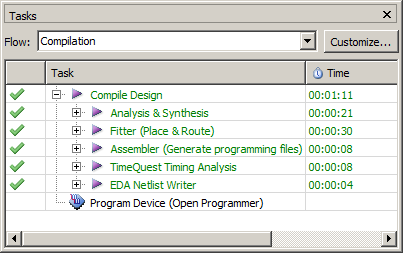
\includegraphics[scale=0.44]{012exampleflow.png}
  \caption{An example of a completed design flow.}
  \label{012exampleflow}
\end{figure}

The script is written in Tcl (''tickle''). Tcl is a \textit{scripting language},
a language designed for automating tasks which could be done by hand by an
human operator. The language provides a full set of flow control statements,
functions and a lot of routines (in Tcl they all are called commands). For a
introductory course on Tcl, see~\cite{web/intro_tcl} and~\cite{book/pptcltk}.

The Quartus environment heavily uses Tcl for scripting purposes and provides a
set of packages. The packages provide an interface to Quartus' internal
information. The script makes use of the \texttt{::quartus::project} Tcl
package. More information can be found in~\cite{web/pkg_quartus_project}.
Examples are: finding the top level design name, the project directory. For an
extensive overview and examples, see~\cite{pdf/scripting_quartus} and~%
\cite{web/example_quartustcl}.

The script makes use of the \texttt{quartus\_map} command. This command is
able to do a lot of  things for you: create the design database, convert files,
analysis and synthesis. See Quartus AN309\textsuperscript{citation needed}.

When the script runs, it prints information in the System tab of the Message
window. This is done by the \texttt{post\_message} command, optionally
followed by a message type. An example of some output can be seen in Figure~%
\ref{015examplemessage}.

Note there's no way to pass arguments to the script, so you can't pass the
name of the ModelSim command file. That's why the script always presumes a
filename as described in Section~\ref{sec:projsetup}.

\begin{figure}[!h]
  \centering
  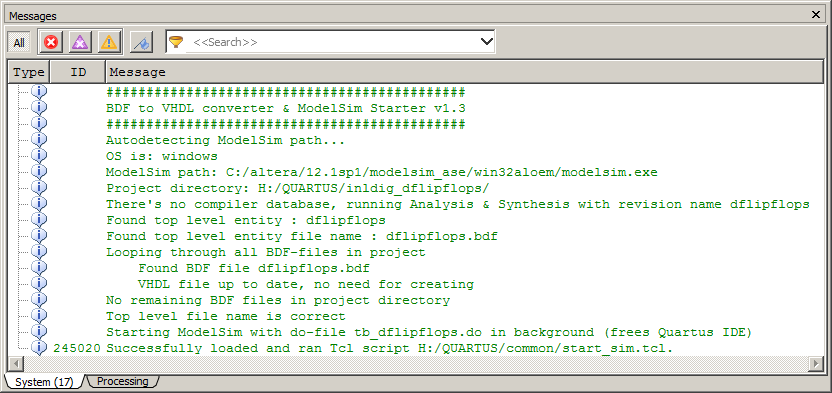
\includegraphics[scale=0.44]{015examplemessage.png}
  \caption{An example output of the script.}
  \label{015examplemessage}
\end{figure}

%%Some of the language constructions could surely be written more compact. But
%%we chose for clarity instead of compact code.

%%%%%%%%%%%%%%%%%%%%%%%%%%%%%%%%%%%%%%
\section{Quick overview of the script}
%%%%%%%%%%%%%%%%%%%%%%%%%%%%%%%%%%%%%%
\label{sec:overview}
This script does a number of things, but mainly it converts all BDF files in
the current project environment into VHDL files and starts ModelSim with an
associated command file. Of course there are a lot of build-in checks to
determine if conversion and simulation is at all possible. A list of stages
is given below:

\begin{enumerate}
\item Checks if the project is open.
\item Finds ModelSim execution path if none is provided. Linux and Windows
      supported.
\item Creates a project database if none is found.
\item Finds the top level entity name, checks if the top level entity name has
      an associated file, complains if none is found.
\item Loops through all BDF files found in the project environment and creates
      associated VHDL files if needed.
\item\label{item:remove}
      Removes all VHDL files from associated BDF files in the project
      directory but not in the project environment, but not VHDL files that do
      NOT have a associated BDF file\footnote{You probably have to read this
      sentence twice. See Section~\ref{sec:internal} for details.}
\item Finds top level filename and creates DO filename.
\item Starts ModelSim with DO filename.
\end{enumerate}


%%%%%%%%%%%%%%%%%%%%%%%%%%%%%%%%%%%%%%%
\section{The Script's Internal Working}
%%%%%%%%%%%%%%%%%%%%%%%%%%%%%%%%%%%%%%%
\label{sec:internal}
For the impatients: a complete printout of the script can be found in
Appendix~\ref{app:completescript}. \\

The script starts with a lot of comment explaining the working of the script
in shorthand. The script is unable to handle arguments due to the fact that it
is called as part of a flow by the Quartus GUI. There is only one user option
available as you can see in Listing~\ref{code:modelsimpath}. If you don't want
the script to find the ModelSim install path, please fill in the user option.

\lstinputlisting[language=tclfix,firstline=45,lastline=47,caption=Set ModelSim path.,label=code:modelsimpath]{start_sim.tcl}

Just as any script, it first prints a pretty banner. Currently, we have
version 1.3 available. See Listing~\ref{code:printbanner}.

\lstinputlisting[language=tclfix,firstline=49,lastline=52,caption=Print a nice banner.,label=code:printbanner]{start_sim.tcl}

In the first stage, the script checks if there is there is an opened project.
It is needed to continue. If there's no opened project, the script exits with
a failure. This can be seen in Listing~\ref{code:openproject}. (Here you can
see an example of Quartus' API, \texttt{is\_project\_open} is a function of the
project package.) For more information, see~\cite{web/pkg_quartus_project}.

\lstinputlisting[language=tclfix,firstline=54,lastline=58,caption=Check for open project.,label=code:openproject]{start_sim.tcl}

Next, the script tries to find the install path of the ModelSim executable if
the user left the install path option blank. First, the Quartus user
environment is consulted and if this is not set, the script searches the
Quartus installation directory for the ModelSim installation. This means
that you have to install ModelSim somewere under the Altera root install path.
Currently, the script can handle Windows and Linux systems. The script will
use the ModelSim Starter Edition, even if it finds more than one ModelSim
installation. The script bails out if it cannot find a ModelSim installation.

%% You can
%%override the automatic detection for the install path by providing a complete
%%path (including the ModelSim excutable name) in the user option
%%\texttt{modelsim\_exec\_path}, e.g., \newline
%%
%%\noindent
%%\texttt{set modelsim\_exec\_path \textbackslash}
%%
%%\texttt{"/opt/altera/12.1/modelsim\_ase/linuxaloem/vsim"} \\
%%
%%\noindent
%%(This is set in source line 46, see the complete listing in appendix
%%\ref{app:completescript}).
This
part is presented in Listing~\ref{code:findmodelsim}%% on page \pageref{code:findmodelsim}
. The found path is then normalized, which means
that references such as \texttt{../} and
\texttt{./} are removed. The path is displayed on screen. \\

\lstinputlisting[language=tclfix,firstline=60,lastline=115,caption=Determine the install path of the ModelSim executable.,label=code:findmodelsim]{start_sim.tcl}

Now, the script checks whether the ModelSim executable is executable. See Listing~\ref{code:checkexec}.

\lstinputlisting[language=tclfix,firstline=118,lastline=122,caption=Check if ModelSim is executable.,label=code:checkexec]{start_sim.tcl}

In the second stage, started in Listing \ref{code:setprojectdir}, the project
directory %%\footnote{On Windows this is called a folder.}
is set. Please read the comment provided
with the code. (Normally, --- the source is the documentation --- should not
hold true, but is this case it's pretty accurate.)

\lstinputlisting[language=tclfix,firstline=124,lastline=133,caption=Set the project directory.,label=code:setprojectdir]{start_sim.tcl}

Next, the script tries to get the top level entity. Normally this is provided
during set up of the Quartus project. If there's no top level entity found,
the script will try to create one. It sets the current revision and starts the
Quartus command \texttt{quartus\_map} with a long list of options. Please note
the \texttt{catch} statement along with the \texttt{exec} statement. When the
command fails, the script issues an error message and exits. The \texttt{catch}
command prevents that. Instead the script prints some information about the
failure of the command. When this happens, there are five possibilities:

\begin{enumerate}
\item You have a project without a file containing the top level description.
Probably a project without design files but with project files.
\item You have a top level design entity that cannot be synthesized, e.g.
testbenches or high level descriptions used for simulation only.
\item You have an error in one of your design files.
\item If the current device is not supported in the current version of Quartus,
the analysis will fail.
\item If you stripped the project of all non-essential files and at startup you
change the device, and the previous device files are not installed, the
analysis will fail.
\end{enumerate}

\noindent
In case of the second item, you can simply restart the script, because now
there is a database and a top level design entity is available.
In case of the fourth and fifth item, you handle as follows:
\begin{itemize}
\item Close Quartus.
\item Open de directory of your Quartus project.
\item Remove the file \texttt{defaults.qdf}.
\item Remove de \texttt{db} and \texttt{incremental\_db} directories.
\item Restart Quartus and open your project.
\end{itemize}

\noindent
The code is presented in Listing~\ref{code:checkdatabase}.

\lstinputlisting[language=tclfix,firstline=135,lastline=160,caption=Check the current revision and database.,label=code:checkdatabase]{start_sim.tcl}

At the fourth stage, the script tries to find the file containing the top level
entity. It does this in three steps. It first finds the top level entity
currently focused, then it finds the associated file containing top level
entity and last it checks if the file really exists. When it fails, there
is no file (you probably deleted it), but the project has a database. You
have to enter a file. See Listing~\ref{code:findtoplevel}.

\lstinputlisting[language=tclfix,firstline=162,lastline=177,caption=Find the file containing top level entity.,label=code:findtoplevel]{start_sim.tcl}

In Listing~\ref{code:allbdffiles}, all BDF filenames in the project are saved
(this will be later explained). Then we print a nice line about what we are
going to do.

\lstinputlisting[language=tclfix,firstline=179,lastline=183,caption=Create a list of all BDF files in the project directory.,label=code:allbdffiles]{start_sim.tcl}

Now we come the the stage where the BDF files are converted to VHDL files
(see Listing~\ref{code:convertbdftovhdl}).
This is a bit tricky to explain, but here is how it works. The project \textit{directory}
contains all files on disk, whereas the project \textit{environment} contains only the
files that were added to the Quartus project as seen in the Project Navigator
window in the Quartus IDE.

The script loops through all the BDF files that were added to the project
environment (these are the files that you want to be in the project). All
these filenames are requested through the Quartus API. The filenames found
are saved in a list for later use (we want them to be converted) but at the
same time the filenames are removed from the list of all BDF files in the project
directory. This way we have a list of all the BDF files we want to convert
and we have list of BDF files that are in the project directory but not in
the project environment (these files are somehow saved in the directory but
are not used in the project).

\lstinputlisting[language=tclfix,firstline=185,lastline=237,caption=Create VHDL files.,label=code:convertbdftovhdl]{start_sim.tcl}

Obviously, you don't want the last set of files
to be converted (maybe you would, but then you have to add them to the project
environment). Rationale for this is that we have students who create a lot
of BDF files and then discard them from the project environment but forget
them to delete. Note that this is done in just a few lines of code directly
under the \texttt{foreach\_in\_collection} command.

Next, the script checks if the file is outside of the project directory. If
the file is outside the project directory, a warning message is issued and the
file is skipped for processing.

The last part of this stage converts the BDF files to VHDL files, but it
only has to be done if the VHDL does not exists or if the VHDL file is
outdated. This last one means that the BDF file was changed after the
corresponding VHDL was created by the script. If a VHDL file should be
created, the script starts a \texttt{quartus\_map} command with the
appropriate options.

At this point (this is the sixth stage), we have a list of all the BDF files
that are not in the project environment (and hence they are not used by
Quartus). All the corresponding VHDL files should be removed so that ModelSim
will not accidentally use them during simulation. See Listing~%
\ref{code:removevhdl}.

Obviously, this should be done by the users, but remind that this script was
intentionally written to support students as an aid for learning digital design
and not for learning how to use ModelSim.

By deleting all unwanted VHDL files we can set up a ModelSim command script
containing a fine piece of code for including all VHDL files. See Listing~%
\ref{code:modcommand} on page~\pageref{code:modcommand}.

\lstinputlisting[language=tclfix,firstline=239,lastline=258,caption=Remove all VHDL files for which a BDF file exists but not in the project environment.,label=code:removevhdl]{start_sim.tcl}

The last two stages can best be seen in one view, as seen in Listing~%
\ref{code:checkstart}. For simulation to start, the filename where the top
level entity resides should be the same as the name of the top level
entity (For BDF files, the entity name is the same as the filename without
the extension.) This is first checked, and the script issues an error if
the check failed. By convention, and because the script
can't handle command line arguments, the name of the command file that is
passed as argument to ModelSim consists of the concatenation of the prefix
\texttt{tb\_} followed by the name of the top level entity name and the extension
\texttt{.do} (this is the default extension for ModelSim command files).
Then, if the command file exists, ModelSim is started. Please
note the '\&' at the end of the \texttt{exec} command. Doing this will prevent
the execution of ModelSim to freeze the Quartus IDE. Of course, when the
test fails, an error is issued.
%% (The filename of the top level entity could
%%be anything you want but the rationale for this is that the student will
%%learn how to use filenaming in a project.)

\lstinputlisting[language=tclfix,firstline=260,lastline=288,caption=Check the top level and start ModelSim.,label=code:checkstart]{start_sim.tcl}

Note that if the user provides a ModelSim command script via the Assignments menu,
this script is used instead of the precomputed script.
 

%%%%%%%%%%%%%%%%%%%%%%%%%%%%%%%%%%%%%%%%%%%%
\section{Setting up a ModelSim command file}
%%%%%%%%%%%%%%%%%%%%%%%%%%%%%%%%%%%%%%%%%%%%
\label{sec:modelsimcommandfile}
The ModelSim command file must contain all commands needed to fulfil the simulation.
Normally, Quartus has the (annoying) habit of creating a few commands by itself
and save them in a file with a strange name before it calls your command file.
You can include compile command for every VHDL file the project
contains, but as files are added or deleted, it is easy to include the code of
Listing~\ref{code:modcommand}. This \texttt{foreach} loop compiles all VHDL
files in the currect directory, which means it will also compile VHDL files
that do not have an associated BDF file.

\begin{lstlisting}[language=tclfix,caption=Including all VHDL Files in a Modelsim Command File.,label=code:modcommand]
foreach vhd_file [ glob *.vhd ] {
	puts "Compiling: $vhd_file"
	vcom -2008 -work work $vhd_file
}
\end{lstlisting}

When displaying signals, please note that the conversion create hierarchical
names consisting of the prefix \texttt{b2v\_} and
the \textit{instantiation name}. Figure~\ref{010convertbdftohdl} shows some
of the sub designs  with  instantiation names (actually, they are library
elements).

So if you have a top level design entity called \texttt{full\_adder} with
a sub design entity called \texttt{xor} and the \texttt{xor} is instantiated
with the name \texttt{inst} (the default, if you have more than one sub designs,
they are called \texttt{inst1}, \texttt{inst2} etc.), using an internal signal
\texttt{inva}, the signal in the xor design are labelled
\texttt{full\_adder/b2v\_inst/inva} in ModelSim. 

%%%%%%%%%%%%%%%%%%%%%%%%%%%%%%%%%%%%%%%%%%%%%%%%%%%%%%%%%%%%%
\section{Installation and use of the script in a design flow}
%%%%%%%%%%%%%%%%%%%%%%%%%%%%%%%%%%%%%%%%%%%%%%%%%%%%%%%%%%%%%
\label{sec:installation}
Installation of this script as a item in a so-called \textit{ design flow}
is not complicated. You can create a flow by hand or use the example file
in Listing~\ref{code:tmf}.
Creating a design flow is discussed in ()\textsuperscript{still not found}.

First, you should save the script in a directory. As you can see at the end
of the Listing, we use
\texttt{H:{\textbackslash}QUARTUS{\textbackslash}common} and name the
script \texttt{start\_sim.tcl} (the first version of the script just
started the simulator as a test). The complete script can be found
in Appendix~\ref{app:completescript}.

Then, simply create a file named \texttt{tmwc\_BDF\_Conversion\_And\_Simulation.tmf}
(mind the extension) using a text editor and copy the the code from Listing
\ref{code:tmf} in Appendix~\ref{app:completescript} into the file. Then move
the file into your Windows profile
directory, which is usually something like 
\texttt{C:{\textbackslash}users{\textbackslash}<your\_name>}.
On Linux you have to place the file in a directory called
\texttt{.quartus.altera} which is generated in
your home directory when you start Quartus for the first time.

Note that the first part of code contains some predefined tasks such as
synthesis, fitter and timing analyser. The second part of the code describes
the whereabouts of the script. Please mind the code fragment where the path
of the script is presented. It should match the path where you placed the
script. Note: do \textit{not} include whitespaces in the script's path!

Appendix \ref{app:installscript} shows an example Windows Visual Basic script to
automatically install the script and the design flow file in the user's profile
directory.
% It will also install a Quartus initialization file found in
%Appendix \ref{app:quartusinifile}.

\lstinputlisting[language=XML,label=code:tmf,caption=The Design Flow File]{tmwc_BDF_Conversion_And_Simulation.tmf}

After you installed the appropriate files, you just simple start the
Quartus software and select the BDF design flow from the Tasks pane.
See Figure \ref{020useofdesignflow}.

\begin{figure}[h!]
  \centering
  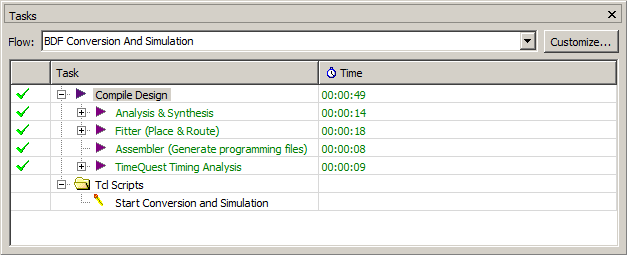
\includegraphics[scale=0.44]{020useofdesignflow.png}
  \caption{The BDF Conversion And Simulation Design Flow.}
  \label{020useofdesignflow}
\end{figure}


%%%%%%%%%%%%%%%%%%%%%%%%%%%%%%%%%%%%%%%%%%%%%%
\section{Things to Remember}
%%%%%%%%%%%%%%%%%%%%%%%%%%%%%%%%%%%%%%%%%%%%%%
\label{sec:remember}
Please note the following when creating your schematics:
\begin{itemize}[itemsep=0pt]
\item Do \emph{not} use VHDL constructs and keywords anywhere in the
schematics. This applies to anything that may render the created VHDL files
containing unwanted and probably illegal VHDL constructs, such as keywords,
entity names and expressions. Examples are: \texttt{is},
\texttt{in}, \texttt{out}, \texttt{of}, \texttt{signal}, \texttt{A<B}.
\item Try to avoid uppercase characters, especially is names for input and
output pins. VHDL is case insensitive (and so is ModelSim), but the pin
planner isn't.
\end{itemize}

%%%%%%%%%%%%%%%%%%%%%%%%%%%%%%%%%%%%%%%%%%%%%%
\section{Known Issues}
%%%%%%%%%%%%%%%%%%%%%%%%%%%%%%%%%%%%%%%%%%%%%%
\label{sec:issues}
There are some known issues, which are all caused by the Quartus
environment.
\begin{itemize}[itemsep=0pt]
\item If you change the top level design entry and run the script directly after
that, the script will find the previous selected top level design entry as
the current one. The workaround is simple: just
rerun Analysis and Synthesis first and you'll be fine.
\item Currently the script can't handle BDF files outside the project directory.
The problem is that the Quartus command \texttt{quartus\_map} has no option
to specify the output directory. It just uses the directory of the input
file. This can interfere with VHDL files in that directory.
\item The script also can't handle library elements because of the aforementioned
problem. (Note that the use of Mega Functions en MAXII functions is not
tested.)
\item Output from the script is first seen when ModelSim starts. Before that, all
output is apparently internally buffered. This is annoying, but up till now
there's no remedy for that.
\item If a component in your design has an unused output (e.g., a carry out of
the most significant bit of a full adder), Quartus will not generate an output
signal in the VHDL file, hence you cannot use the signal in ModelSim.
\end{itemize}

\newpage
\appendix
\section{The Complete Tcl Script}
\label{app:completescript}
The complete script can also be downloaded from \url{http://ds.opdenbrouw.nl/quartus}.
%%presented here is the complete script. You should copy the text using a
%%standard text editor into a Tcl file, a file that has the extension \texttt{.tcl}.
\lstinputlisting[language=tclfix,numbers=none,caption=The Complete Script.,label=code:complete]{start_sim.tcl}

\newpage
\section{The Design Flow File}
\label{app:completeflowfile}
The complete design flow file can also be downloaded from \url{http://ds.opdenbrouw.nl/quartus}.
\lstinputlisting[language=XML,numbers=none,label=code:completeflow,caption=The Design Flow File]{tmwc_BDF_Conversion_And_Simulation.tmf}

\newpage
\section{An Example of a Install Script on Windows}
\label{app:installscript}
%\lstinputlisting[language=command.com,numbers=none,label=code:installcmd,caption=An Example of a Install Script on Windows]{install_flow.cmd}
\lstinputlisting[language=VBScript,numbers=none,label=code:installcmd,caption=An Example of a Install Script on Windows]{install_flow.vbs}

\newpage
%%\section{An Example of a Quartus Initiazation File}
%%\label{app:quartusinifile}
%%\lstinputlisting[numbers=none,label=code:quartusini,caption=An Example of a Quartus Initiazation File]{quartus2.ini}

\newpage
\section{Changelog \& To Do}
\label{app:changelogandtodo}
Changelog to the documentation:

\begin{itemize}\itemsep0pt
\item[]22-01-2014: Added failure feature 4 and 5 if analysis fails.
\item[]05-03-2014: Changed TMF file name to reflect the fact that BDF files
                   are converted.
\item[]08-03-2014: Minor spelling corrections.
\item[]09-03-2014: New screenshot BDF Conversion And Simulation
\item[]19-09-2018: Updated the script, changed command batch file for VBscript, typos.
\item[]27-08-2021: Update the script and documentation.
\end{itemize}


%\bigskip\bigskip
%\noindent
%To Do Documentation and Script:
%\begin{itemize}\itemsep0pt
%\item It is possible to use the \texttt{EDA\_SIMULATION\_RUN\_SCRIPT} global
%      assignment. This way, the user
%      can supply a do-file instead of using the predefined names with the
%      prefix \texttt{tb\_}.
%\end{itemize}




\newpage
%\bibliographystyle{plain}
%\bibliography{convertBDFtoVHDL}
\printbibliography

\end{document}